%# -*- coding: utf-8-unix -*-
% !TEX program = xelatex
% !TEX root = ../thesis.tex

\chapter{Recommendation Algorithms}

    \todo{chapter intro}

\section{Random Policy}

    \todo{all kinds of baselines}

\section{Reinforcement Learning}

    \subsection{Environment}

        We encapsulate the recurrent neural network user model into a reinforcement learning environment.
        The environment provides APIs similar to the OpenAI Gym \cite{brockman_openai_2016}.

        \verb|env = Environment(lookback)| returns an instance of the reinforcement learning environment,
        with the specified \verb|lookback| hyper-parameter for the recurrent neural network.

        \verb|observation = env.new_episode()| asks the environment to start a new episode and return the initial observation.
        The initial state is constructed from a randomly picked submission of the Online Judge data set.
        It simulates the mindset of the user when making the picked submission.

        At the beginning of an episode, the environment also calculates the ``user score''.
        We define the user score as the average of the probabilities of the user able to solve each problem.
        An observation from the environment is exactly the user features part of the whole input vector for the user model.
        Thus, the way to estimate the probability of the user able to solve a given problem
        is to ask the user model to predict the input concatenated by the state and the corresponding problem features.

        \verb|observation, reward, done = env.step(action)|
        demands the environment to simulate the process of the user solving the given problem.
        An \verb|action| can be one-to-one mapped to a problem.
        It returns the new observation vector, the reward scalar, and whether the episode has finished or not.

        The environment simulates the process of the user solving the given problem in the following manner.
        The environment asks the user model to predict the probability $p$ of the user able to solve the problem.
        Then, it samples the number of attempts $n$ before the user successfully solves the problem
        from the geometric distribution $n \sim \mathrm{Geometric}(p)$.
        Next, the environment updates the relevant counting features
        as if the user has made $n-1$ unsuccessful submissions followed by one accepted solution.
        The new user feature is returned as the new observation.
        Finally, the environment recalculates the user score.

        We define the reward as the difference from the current user score to the previous one.
        Hence, the return $R_t$ of the reinforcement learning agent
        would be the expected total increment of user score in the future,
        if the discount factor $\gamma$ is set to 1.
        An episode ends after solving 50 problems.

    \subsection{Implementation}

        We implemented the A3C algorithm with the \verb|Keras|\cite{chollet2015keras} Python library.

    \subsection{Result}

        We trained the A3C agent with 32 cores.
        It converged within an hour.
        The improvement on user score is shown in Figure \ref{fig:a3c-episode-reward}.
        \begin{figure}[!htp]
            \centering
            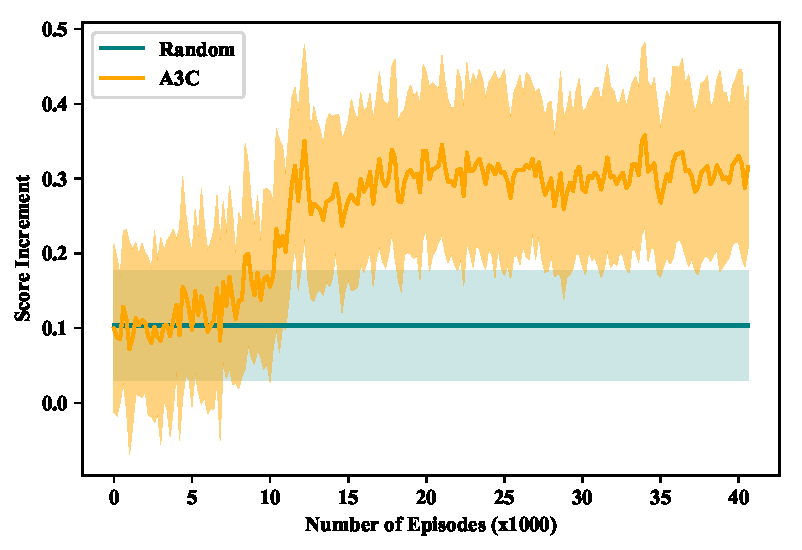
\includegraphics[width=0.62\textwidth]{img/a3c-episode-reward.pdf}
            \caption{Rewards of the A3C agent during the training process}
            \label{fig:a3c-episode-reward}
        \end{figure}









